\documentclass[a4paper, oneside]{report}

\usepackage[top=3cm, bottom = 3cm, left = 3cm, right =3cm]{geometry}
\usepackage{amsfonts,amsmath,amssymb}
\usepackage[utf8]{inputenc}
\usepackage[francais]{babel}
\usepackage{graphicx}
\usepackage{polynom}
\usepackage[T1]{fontenc}
\usepackage{mathenv}
\usepackage{array}
\usepackage{mdwtab}
\usepackage[colorlinks=true,linkcolor=black]{hyperref}
\frenchbsetup{StandardLists=true}
\usepackage{listings}
\usepackage{xcolor}
\usepackage{graphicx}
\usepackage{tikz}
\usepackage{circuitikz}
\usetikzlibrary{arrows,automata}
\definecolor{darkgreen}{rgb}{0, 0.6, 0}
\lstset{language=caml, frameround = fttt}

\lstset{upquote=true,
        columns=flexible,
        keepspaces=true,
        breaklines,
        breakindent=0pt,
        basicstyle=\ttfamily,
        breaklines=true,
        keywordstyle=\color{red},
        commentstyle=\color{darkgreen},
        tabsize=2,
        escapechar={¤},
        escapebegin=\color{gray},
        }


\newcommand{\adb}{arbre~de~décision binaire~}
\newcommand{\adbs}{arbres~de~décision binaires~}
\newcommand{\adbo}{\adb ordonné~}
\newcommand{\adbos}{\adbs ordonnés~}
\newcommand{\adboc}{\adbo canonique~}
\newcommand{\adbocs}{\adbos canoniques~}
\newcommand{\expp}{expression~propositionnelle~}
\newcommand{\expps}{expressions~propositionnelles~}
\newcommand{\ssi}{si~et~seulement~si~}

\begin{document}


\title{Arbre de décision binaire - \textit{ROBDD} en anglais \\ Rapport pour le projet Mathématique et Informatique de L3 de 2018-2019  }
\date{\today}
\author{Sébastien Palmer et Xavier Durand \\~\\ Encadré par Sedki Boughattas }
\maketitle

\tableofcontents{}

\newpage

%%%%% INTRODUCTION %%%%%%%
\chapter*{Introduction}
\addcontentsline{toc}{chapter}{Introduction}

\section*{Présentation du sujet}
Ce document est un projet de Mathématiques et d'Informatique suivi et encadré par un enseignant chercheur à l'Université Paris Diderot.\\
Nous allons ici traiter des arbres de décisions binaires. Le projet se base sur l'article de Henrik Reif Andersen \og\textit{An Introduction to Binary Decision Diagrams}\fg{}.\\
Ce document traite de ce qu'est un arbre de décision binaire, et de la représentation de toutes expressions propositionnelles en un arbre de décision binaire. Enfin, il expose un algorithme permettant de construire l'\adb correspondant à une expression propositionnelle quelconque.\\

\section*{Qu'est ce qu'une expression propositionnelle}

Dans un premier temps, on va présenter ce qu'est une expression propositionnelle.\\
\subsubsection*{Variable propositionnelle}
Une variable propositionnelle correspond à une variable comme en Mathématiques. Cependant, son ensemble de définition correspond à l'ensemble $\{0,1\}$, où ici on peut apparenter $0$ à \textit{faux} et $1$ à \textit{vrai}.\\
Pour lier différentes variables propositionnelles entre elles, on va introduire des connecteurs logiques.
\subsubsection*{Connecteurs logiques}
On va présenter ici les cinq symboles logiques les plus utilisés en logique propositionnelle :
\begin{itemize}
\item la négation : on la notera $\neg$. Elle correspond à une fonction ne prenant qu'une expression propositionnelle en argument et renvoie vrai \ssi l'argument est faux.

\item la conjonction : on la notera $\wedge$. Elle correspond à une fonction prenant deux \expps en argument et renvoie vrai \ssi les deux arguments sont vrais. 

\item la disjonction : on la notera $\vee$. Elle correspond à une fonction prenant deux \expps en argument et renvoie faux \ssi les deux arguments sont faux (donc renvoie vrai si au moins l'un des deux arguments est vrai).

\item l'implication : on la notera $\Rightarrow$. C'est une fonction prenant deux \expps en arguments et renvoyant faux \ssi le premier argument est vrai et le deuxième est faux.

\item l'équivalence : on la notera $\Leftrightarrow$. C'est une fonction prenant deux \expps en argument et renvoyant vrai \ssi les deux arguments ont la même valeur de vérité.

\end{itemize}

\newpage

Voici les tables de vérités de chacun des connecteurs logiques :
\begin{figure}[h]
\begin{center}
\begin{tabular}[t]{|c|c|}
\hline 
 & $\neg$ \\ 
\hline 
$0$ & $1$\\
$1$ & $0$ \\ 
\hline 
\end{tabular}
\hspace*{1em}
\begin{tabular}[t]{|c|cc|}
\hline 
$\wedge$ & $0$ & $1$ \\ 
\hline 
$0$ & $0$ & $0$\\
$1$ & $0$ & $1$ \\ 
\hline 
\end{tabular}
\hspace*{1em}
\begin{tabular}[t]{|c|cc|}
\hline 
$\vee$ & $0$ & $1$ \\ 
\hline 
$0$ & $0$ & $1$\\
$1$ & $1$ & $1$ \\ 
\hline 
\end{tabular}
\hspace*{1em}
\begin{tabular}[t]{|c|cc|}
\hline 
$\Rightarrow$ & $0$ & $1$ \\ 
\hline 
$0$ & $1$ & $1$\\
$1$ & $0$ & $1$ \\ 
\hline 
\end{tabular}
\hspace*{1em}
\begin{tabular}[t]{|c|cc|}
\hline 
$\Leftrightarrow$ & $0$ & $1$ \\ 
\hline 
$0$ & $1$ & $0$\\
$1$ & $0$ & $1$ \\ 
\hline 
\end{tabular}
\end{center}
\caption{Tables de vérités des cinq connecteurs logiques}
\end{figure}

Ces connecteurs logiques ne sont bien évidemment pas les seuls à exister, mais ce sont ceux qu'on accepte dans notre algorithme qu'on présentera plus tard.

\subsubsection{Expression propositionnelle}
Une \expp correspond à une suite de variables propositionnelles liées par des connecteurs logiques.\\
Voici un exemple d'\expp :
$$(x \wedge y) \vee ((\neg z) \Rightarrow (x \Leftrightarrow t))$$
avec $x,y,z$ et $t$ des variables propositionnelles.\\

Par soucis de lisibilité, lorsqu'on écrira une expression propositionnelle, on ajoutera des parenthèses.\\
Prenons l'expression $x\wedge y\vee 1$. On ne va pas avoir la même table de vérité si on écrit $(x\wedge y)\vee 1$ (qui sera toujours vrai) et si on écrit $x \wedge (y \vee 1)$ (qui sera faux si $x$ est faux).\\
Cependant, il y a des expressions qui sont commutatives, et donc on peut omettre les parenthèses dans ces cas précis. Ces expressions commutatives sont la succession de conjonction et la succession de disjonction. Les tables de vérité des deux \expps suivantes ne change pas quelque soit la position des parenthèses :
$$x \wedge y \wedge z \hspace{2em} et \hspace{2em} x \vee y \vee z$$

\section*{Qu'est ce qu'une ROBDD (présentation rapide)}

\noindent Nous allons ensuite introduire la notion d'arbre de décision binaire, on le notera \textit{ADB}. Cela se présente de la sorte :

\begin{figure}[htbp]
  \centering
  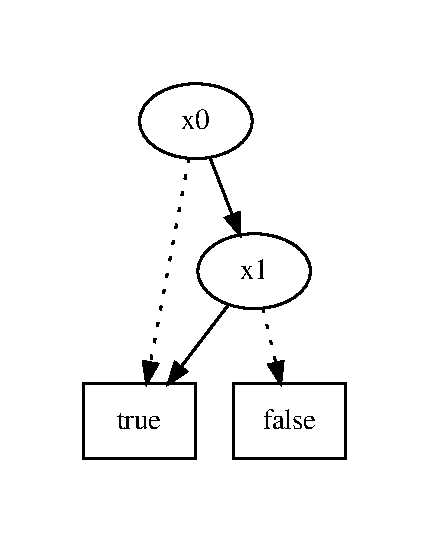
\includegraphics[trim = 0cm 1.5cm 0cm 1cm , scale=0.6]{exemple/impl_simple}
  \caption{ADB d'un implication simple : $x_0 \Rightarrow x_1$}
\end{figure}
Cet arbre se lit de haut en bas : on commence par évaluer la première variable, soit à $vrai$ soit à $faux$. Ensuite on arrive dans un autre état où la première variable n'existera plus et sera remplacé par son évaluation.\\
On réitère ensuite ce processus pour les variables qui suivent.\\
La flèche en pointillée représente le chemin à emprunter si la variable correspondant au nœud a 0 pour valeur de vérité et la flèche pleine correspond à la valeur de vérité 1.\\
Ici, on voit bien que si $x_0$ est faux, alors l'implication est vrai, quelque soit la valeur de vérité de $x_1$.\\
Si $x_0$ est vrai, alors il faut regarder la valeur de vérité de $x_1$ : si $x_1$ est vrai, alors l'implication est vraie et si $x_1$ est faux alors l'implication est fausse.\\

Ici, on a aussi introduit l'idée que cet arbre est ordonné, qu'on notera \textit{ADBO} (arbre de décision binaire ordonné).\\
Il faut donner un ordre aux variables pour savoir dans quel ordre on va attribuer une valeur de vérité aux variables pour former l'arbre.\\
On le présentera plus en détail plus tard, mais il s'avère que l'arbre dépend de l'ordre choisi : on peut obtenir un arbre plus petit avec un certain ordre et un autre beaucoup plus grand avec un autre ordre.\\

Enfin, introduisons la notion d'unicité de cet arbre. La construction de l'arbre est unique en fonction de l'ordre choisi, c'est à dire qu'en ayant fixé un ordre, toutes les expressions équivalentes posséderont le même ADB. On le notera \textit{ADBOC} (arbre de décision binaire ordonné canonique).\\
 
\section*{Organisation}
On va ici vous présenter les résultats de notre recherche sur le sujet.\\
Dans un premier temps, on va vous présenter les propriétés d'un ADBOC et la raison pour laquelle on peut générer pour toutes \expps un ADBOC.\\
Ensuite, nous présenterons l'algorithme que nous avons implémenté en Ocaml pour pouvoir générer ces ADBOCs. Nous discuterons aussi de la complexité de cet algorithme.\\
Enfin, nous présenterons les intérêts des ADBOCs ainsi que des réflexions qu'on peut avoir sur leurs utilisations.  



%%%%% Chapitre 1 %%%%%%%
\chapter{Représentation sous ROBDD}

\section{Opérateur If-then-else et INF}

Soit $ x \rightarrow y_0, y_1 $ l'opérateur \textit{if-then-else} défini par \\
$$ x \rightarrow y_0, y_1 = ( x \wedge y_0 ) \vee ( \neg x \wedge y_1 )$$
Ainsi, $ t \rightarrow t_0, t_1 $ est \textit{vrai} si $t$ et $t_0$ sont \textit{vrais} ou si $t$ est \textit{faux} et $t_1$ est \textit{vrai}, et est faux sinon.\\
Tout les operateurs peuvent assez facilement être traduits en utilisant uniquement l'opérateur \textit{if-then-else}, 1 et 0 (Pour \textit{vrai} et \textit{faux}) :\\

\begin{itemize}
\item $ \neg A = A \rightarrow 0, 1$
\item $ (A \wedge B) = A \rightarrow B, 0$
\item $ (A \vee B) = A \rightarrow 1, B$
\item $ (A \Rightarrow B) = A \rightarrow B, 1$
\item $ (A \Leftrightarrow B) = A \rightarrow B, (B \rightarrow 0, 1)$
\end{itemize}

où $A$ et $B$ sont des variables propositionnelles.\\

On peut aussi représenter une variable propositionnelle $A$ par $A \rightarrow 1, 0$

On introduit donc la \textit{Forme Normale If-then-else} (INF : \textit{If-then-else Normal Form}) comme étant une expression Booléenne construite entièrement avec l'opérateur \textit{if-then-else}, 1 et 0 appliqué aux variables propositionnelles de la formule qu'elle traduit.\\

En notant $t[0/x]$ l'expression obtenu en remplaçant la variable $x$ par $0$ dans $t$, on remarque assez facilement que :
$$ t = x \rightarrow t[1/x], t[0/x] $$ pour chaque variable de t.\\
On appelle se résultat l'\textit{Expansion de Shannon} de $t$ sur $x$.

Grâce à ce résultat, on peut générer, pour chaque expression booléenne, une INF en réitèrant l'expansion de Shannon sur chaque variable de l'expression.

On a vu précédement que toute expression Booléenne est équivalente à une expression en INF, on a maintenant un moyen de la trouver.\\

Exemple : Soit $t = ( x_1 \Leftrightarrow y_1 ) \wedge ( x_2 \Leftrightarrow y_2 )$.\\
On peut donc appliquer l'expansion de Shannon :
\begin{center}
$t = x_1 \rightarrow t_1, t_0)$\\
$t_0 = y_1 \rightarrow 0, t_{00})$\\
$t_1 = y_1 \rightarrow t_{11}, 0)$\\
$t_{00} = x_2 \rightarrow t_{001}, t_{000})$\\
$t_{11} = x_2 \rightarrow t_{111}, t_{110})$\\
$t_{000} = y_2 \rightarrow 0, 1)$\\
$t_{001} = y_2 \rightarrow 1, 0)$\\
$t_{110} = y_2 \rightarrow 0, 1)$\\
$t_{111} = y_2 \rightarrow 1, 1)$\\
\end{center}

\section{Les ROBDD et leurs propriétés}

On introduit les \textit{Diagrammes de Décision Binaire} (BDD) définis avec :
\begin{itemize}
\item les noeuds représentant les expressions booléennes t la variable $x$ dans l'expansion de Shannon.
\item Les arêtes en pointillés représentant la valuation de $x$ en $0$ dans l'expansion de Shannon.
\item Les arêtes pleines représentant la valuation de $x$ en $1$ dans l'expansion de Shannon.
\end{itemize}

Ainsi, chaque noeud non-terminal représente une expansion de Shanon $ t = x \rightarrow t_1, t_0 $ et est représenté par un triplet $(var, low, high)$ où :
\begin{itemize}
\item $var$ est $x$
\item $low$ est le noeud représentant $t_0$
\item $high$ est le noeud représentant $t_1$
\end{itemize}

Les noeuds terminaux sont $0$ et $1$\\

On représente donc une expression par le noeud racine.\\

Avec l'exemple précédent, on obtient le BDD suivant :

\newcommand{\largeur}{0.5\linewidth}

\begin{figure}[h]
      \begin{tikzpicture}[shorten >=1pt,node distance=1cm]
\node[state]		   (X1) at (0,4)         {$x_1$};
  \node[state]		   (Y11) at (-1,3)         {$y_1$};
  \node[state]		   (Y12) at (1,3)         {$y_1$};
  \node[state]		   (X21) at (-2,2)         {$x_2$};
  \node[state]		   (X22) at (2,2)         {$x_2$};
  \node[state]		   (Y21) at (-4,1)         {$y_2$};
  \node[state]		   (Y22) at (-2,1)         {$y_2$};
  \node[state]		   (Y23) at (2,1)         {$y_2$};
  \node[state]		   (Y24) at (4,1)         {$y_2$};
  \node[state, accepting, below]		   (T1) at (-4.5,0)         {$1$};
  \node[state, accepting, below]		   (F1) at (-3.5,0)         {$0$};
  \node[state, accepting, below]		   (F2) at (-2.5,0)         {$0$};
  \node[state, accepting, below]		   (T2) at (-1.5,0)         {$1$};
  \node[state, accepting, below]		   (F3) at (-0.5,0)         {$0$};
  \node[state, accepting, below]		   (F4) at (0.5,0)         {$0$};
  \node[state, accepting, below]		   (T3) at (1.5,0)         {$1$};
  \node[state, accepting, below]		   (F5) at (2.5,0)         {$0$};
  \node[state, accepting, below]		   (F6) at (3.5,0)         {$0$};
  \node[state, accepting, below]		   (T4) at (4.5,0)         {$1$};


  \path[->,>=stealth', dashed] 
		(X1) edge              node {} (Y11)
        (Y11) edge              node {} (X21)
        (Y12) edge              node {} (F4)
        (X21) edge              node {} (Y21)
        (X22) edge              node {} (Y23)
        (Y21) edge              node {} (T1)
        (Y22) edge              node {} (F2)
        (Y23) edge              node {} (T3)
        (Y24) edge              node {} (F6);

  \path[->,>=stealth'] 
		(X1) edge              node {} (Y12)
        (Y11) edge              node {} (F3)
        (Y12) edge              node {} (X22)
        (X21) edge              node {} (Y22)
        (X22) edge              node {} (Y24)
        (Y21) edge              node {} (F1)
        (Y22) edge              node {} (T2)
        (Y23) edge              node {} (F5)
        (Y24) edge              node {} (T4);
    \end{tikzpicture}
\end{figure}

Si les variables apparaîssent dans un même ordre tout au long de la construction du BDD, on dit que le diagramme est \textit{ordonné} (OBDD).\\

On remarque certains noeuds sont dupliqués.\\
Ainsi, dans l'exemple lors de la construction, on réduit par :

\begin{center}
$t_{000} = t_{110}$\\
$t_{001} = t_{111}$\\
$t_{00} = t_{11}$\\
\end{center}

Et on obtient :

\begin{center}
$t = x_1 \rightarrow t_1, t_0)$\\
$t_0 = y_1 \rightarrow 0, t_{00})$\\
$t_1 = y_1 \rightarrow t_{00}, 0)$\\
$t_{00} = x_2 \rightarrow t_{001}, t_{000})$\\
$t_{000} = y_2 \rightarrow 0, 1)$\\
$t_{001} = y_2 \rightarrow 1, 0)$\\
\end{center}

Le diagramme devient donc :\\

\begin{figure}[h]
      \begin{tikzpicture}[shorten >=1pt,node distance=1cm]
\node[state]		   (X1) at (0,4)         {$x_1$};
  \node[state]		   (Y11) at (-1,3)         {$y_1$};
  \node[state]		   (Y12) at (1,3)         {$y_1$};
  \node[state]		   (X2) at (0,2)         {$x_2$};
  \node[state]		   (Y21) at (-1,1)         {$y_2$};
  \node[state]		   (Y22) at (1,1)         {$y_2$};
  \node[state, accepting, below]		   (T) at (0.5,0)         {$1$};
  \node[state, accepting, below]		   (F) at (-0.5,0)         {$0$};


  \path[->,>=stealth', dashed] 
		(X1) edge              node {} (Y11)
        (Y11) edge              node {} (X2)
        (Y12) edge              node {} (F)
        (X2) edge              node {} (Y21)
        (Y21) edge              node {} (T)
        (Y22) edge              node {} (F);

  \path[->,>=stealth'] 
		(X1) edge              node {} (Y12)
        (Y11) edge              node {} (F)
        (Y12) edge              node {} (X2)
        (X2) edge              node {} (Y22)
        (Y21) edge              node {} (F)
        (Y22) edge              node {} (T);
    \end{tikzpicture}
\end{figure}

Si tout noeud redondant a été supprimé et tous noeuds identiques ont été réduits, on dit que le diagramme est \textit{réduit} (ROBDD).\\

Un ROBDD admet donc plusieurs propriétés :

\begin{itemize}
\item Contient un ou deux noeud terminaux ($0$ et/ou $1$)
\item Contient un ensemble de noeuds $u$ non-terminaux de degré 2 ($var(u)$ la variable $x$ du noeud, $low(u)$ le noeud de $t[0/x]$, $high(u)$ le noeud de $t[1/x]$)
\item Les var(u) des noeuds respectent un ordre en fonction de leur place dans le diagramme ($x_1 < x_2 < ... < x_n$)
\item Soit 2 noeuds $u$ et $v$, si $var(u) = var(v)$, $low(u) = low(v)$ et $high(u) = high(v)$ alors $u = v$
\item Soit $u$ un noeud alors $low(u) \neq high(u)$
\end{itemize}

\begin{figure}[h]
      \begin{tikzpicture}[shorten >=1pt,node distance=1cm]
\node 			(N) at (0,3)		{Ordonnée : x < y, x < z};
  \node[state]		   (X) at (0,1.5)         {$x$};
  \node[state]         (Y) at (-1,0)		 {$y$};
  \node[state]         (Z) at (1,0)		 {$z$};


  \path[->,>=stealth', dashed] 
		(X) edge              node {} (Y);
		
  \path[->,>=stealth'] 
        (X) edge              node {} (Z);
	
\end{tikzpicture}
      \begin{tikzpicture}[shorten >=1pt,node distance=1cm]
\node 			(N) at (0,3)		{Unique};
  \node[state]		   (X) at (-1,1.5)         {$x$};
  \node[state]		   (X2) at (1,1.5)         {$x$};
  \node[state]         (Y) at (-1,0)		 {$y$};
  \node[state]         (Z) at (1,0)		 {$z$};

  
  \draw (0.5,1) -- (1.5,2) (0.5,2) -- (1.5,1);
  \path[->,>=stealth', dashed] 
		(X) edge              node {} (Y)
		(X2) edge              node {} (Y);
		
  \path[->,>=stealth'] 
        (X) edge              node {} (Z)
        (X2) edge              node {} (Z);

\end{tikzpicture}
      \begin{tikzpicture}[shorten >=1pt,node distance=1cm]
\node 			(N) at (0,3)		{Non-redondant};
  \node[state]		   (X) at (0,1.5)         {$x$};
  \node[state]         (Y) at (0,0)		 {$y$};

  
  \draw (-0.5,1) -- (0.5,2) (-0.5,2) -- (0.5,1);
  \path [->,>=stealth', dashed, out=210, in=150] 
  (X) edge              node {} (Y);
  
  \path [->,>=stealth', out=-30, in=30] 
  (X) edge              node {} (Y);

\end{tikzpicture}
\end{figure}


\section{Un unique ROBDD pour chaque fonction binaire}

On a vu précédement que l'on peut associer à toute formule propositionnelle un ROBDD.\\

On pose la valuation d'une formule comme une fonction binaire $f :\mathbb{B}^n \to \mathbb{B}$ (où $n$ est le nombre de variable dans la formule).\\

\textbf{Lemme (Canonicité): } Pour toute fonction $f :\mathbb{B}^n \to \mathbb{B}$ il existe exactement un ROBDD $u$ avec comme ordre $x_1 < x_2 < ... < x_n$ notée $f^u = f(x_1,x_2,...,x_n)$

Pour simplifier la démonstration, on pose :\\
\begin{center}
$f_b(x_2,...,x_n) = f(b,x_2,...,x_n)$ où $b \in \mathbb{B}$\\
\end{center}

\textbf{Démonstration } Par induction sur $n$ :\\

Si $n = 0$\\
Alors il n'existe que deux fonctions binaires sans argument : $f = 0$ et $f = 1$.\\
Et il n'y a que deux ROBDD qui n'utilisent pas de variable : $0 (= false)$ et $1 (= true)$\\
Or $0$ est un ROBDD pour $f = 0$ mais pas pour $f = 1$ \\
et $1$ est un ROBDD pour $f = 1$ mais pas pour $f = 0$ \\
Donc il y a un unique ROBDD pour chaque $f :\mathbb{B}^0 \to \mathbb{B}$ \\

Si $n \neq 0$\\
Supposons que le Lemme est vrai pour tout $k <= n$, montrons que le Lemme est aussi vrai pour $n+1$.\\

Soit $f :\mathbb{B}^{n+1} \to \mathbb{B}$.
Alors $f(x_1,...,x_{n+1}) = x_1 \rightarrow f_1(x_2,...,x_{n+1}), f_0(x_2,...,x_{n+1})$\\
Par induction : il y existe des uniques ROBDD $u_0$ et $u_1$ tels que $f^{u_0} = f_0$ et $f^{u_1} = f_1$.\\

Il y a deux cas à considérer :\\

Si $u_1 = u_0$ alors $f_0 = f^{u_0} = f^{u_1} = f_1$ donc $u_0 (= u_1)$ est aussi un ROBDD pour $f$. Qui est aussi unique dû à l'ordre.\\
En effet, si $x_1$ se trouvait dans le ROBDD enraciné dans $u$ alors $var(u) = x_1$.\\
Cependant $f = f^u$ alors $f_0 = f^u[0/x_1] = f^{low(u)}$ et $f_1 = f^u[1/x_1] = f^{high(u)}$ mais $f_0 = f_1$ alors par induction $low(u) = high(u)$ ce qui viole une des propriétés des ROBDD.\\

Si $u_1 \neq u_0$ alors par induction $f_{u_0} \neq f_{u_1}$.\\
Construisons $u$ tel que $var(u) = x_1$, $low(u) = u_0$ et $high(u) = u_1$ ainsi $f^u = x_1 \rightarrow f^{u_1}, f^{u_0}$\\
Par induction $f^{u_1} = f_1$ et $f^{u_0} = f_0$. Or $f(x_1,...,x_{n+1}) = x_1 \rightarrow f_1(x_2,...,x_{n+1}), f_0(x_2,...,x_{n+1})$ donc $f = f^u$ \\
Supposons $v$ un ROBDD tel que $f = f^v$. Clairement $f^v$ dépend de $x_1$. Donc $f^v[0/x_1] \neq f^v[1/x_1]$ (Sinon cela violerait le ROBDD).\\
Grâce à l'ordre $var(u) = x_1 = var(v)$.\\
De plus $f^u = f$ donc $f^{low(v) = f_0 = f^{u_0}}$ et $f^{high(v) = f_1 = f^{u_1}}$ par induction $low(v) = u_0 = low(u)$ et $high(v) = u_1 = high(u)$.\\
Donc par unicité des ROBDD $u = v$


%%%%% Chapitre 2 %%%%%%%
\chapter{Construction d'une ROBDD}

On a implémenté tout un algorithme (en Ocaml) prenant en argument une expression propositionnelle et permettant d'obtenir l'ADBOC de celle-ci.\\
On va vous présenter les fonctions principales.

\section{présentation de l'algorithme}

Il faut déjà comprendre que l'algorithme implémenté est dans un paradigme impératif et qu'on va utiliser une structure correspondante à une Hashmap : l'accès à un élément est linéaire amorti et l'ajout est en temps linéaire amorti, c'est à dire qu'on peut faire ces opérations en temps constant dans un moyenne des temps mais en temps linéaire dans le pire des cas.\\
Notons avant de comprendre l'algorithme en détail que nous avons une structure, noté $S$, qui nous permet d'associer un nœud de l'arbre à ses deux nœuds enfants : on notera \textit{low} pour le nœud suivant la valuation à \textit{faux} et \textit{high} le nœud correspondant à la valuation \textit{vrai} de la variable du nœud parent.\\
Enfin, on indicera les variables par leur rang dans l'ordre : $x_n$ est la $n$-ième variable, $n\in \mathbb{N}$ et $n\geq 0$.\\

L'algorithme est basé sur un principe récursif, on refait la même étape jusqu'à atteindre la condition de fin :
\begin{enumerate}
\item \label{order_eval} On détermine l'ordre d'évaluation des variables en fonction de l'ordre donné, pour obtenir un arbre ordonné.
\item \label{start_eval} On évalue l'\expp donnée en argument pour voir si la valuation n'est pas déjà déterminable. Par exemple, si on a $0 \wedge x$ avec $x$ une variable propositionnelle, alors on sait déjà que quelque soit la valuation de $x$, l'expression est fausse.
\item Si la valuation est déterminée, on renvoie la nœud de l'arbre correspondant à la valeur de vérité correspondante (\textit{vrai} ou \textit{faux}).
\item Sinon, on crée le nœud \textit{low} et le nœud \textit{high} : 
 \begin{itemize}
\item \textit{low} correspond au nœud créé quand on repasse par l'étape \ref{start_eval} où on a remplacé la variable évaluée par $0$ et où on évalue par la variable suivante dans l'ordre de l'étape \ref{order_eval}.
\item \textit{high} correspond au nœud créé quand on repasse par l'étape \ref{start_eval} où on a remplacé la variable évaluée par $1$ et où on évalue par la variable suivante dans l'ordre de l'étape \ref{order_eval}.
\end{itemize}
\item Ensuite, on regarde si le nœud avec comme suivant \textit{low} et \textit{high} n'a pas déjà été créé, auquel cas on le crée, sinon on récupère le nœud déjà créé. Cela permet d'être sur qu'on obtient bien un arbre canonique.
\item Enfin, on renvoie le nœud créé. A la fin de l'algorithme, le dernier nœud renvoyé correspondra à la racine de l'arbre.
\end{enumerate}

\section{Création d'un nœud}

On vous présente en simplifier le code de la fonction qui s'occupe de créer un nouveau nœud en cas de besoin. Ensuite nous commenterons les différentes lignes.
\begin{lstlisting}
let mk (i : indice de la variable) (low : noeud) (high : noeud) : node =
    if low = high then low      (* #1 *)
    else
    if member i low high then   (* #2 *)
      lookup i low high         (* #3 *)
    else
      create_node i low high    (* #4 *)
\end{lstlisting}
On regarde d'abord si on obtient le même résultat quelque soit la valuation de la i-ème variable ($\#1$). Si c'est le cas, on renvoie le nœud correspondant à une des deux valuations (on garde la canonicité).\\
Si ce n'est pas le cas, on regarde si on n'a pas déjà créé un nœud ayant le même \textit{low} et le même \textit{high} ($\#2$), auquel cas on renvoie ce nœud ($\#3$).\\
Enfin, si le nœud n'existe pas, alors on le crée ($\#4$).\\
Dans le meilleur des cas, la création se fait en temps constant et dans le pire des cas, elle se fait en temps linéaire (à cause de la Hashmap).

\section{Construction de l'arbre}

On va ensuite pouvoir exposer l'algorithme correspondant à la construction même de l'arbre.
\begin{lstlisting}
let build (f : exp propositionnelle) : noeud = 
    let tab = Array.init (!n) (function a -> None) in
    let rec aux (f : exp propositionnelle) (i : indice de la variable) : node =
      match getBool f tab with 									(* #1 *)
      | (None, nf) -> begin										(* #2 *)
          if i >= (!n) then failwith "exception de getBool"		(* #3 *)
          else begin
            let v0 = tab.(i) <- (Some false); aux nf (i+1) in	(* #4 *)
            let v1 = tab.(i) <- (Some true); aux nf (i+1) in	(* #5 *)
            tab.(i) <- None;	
            mk i v0 v1											(* #6 *)
          end
        end
      | (Some b, _) -> 											(* #7 *)
        if b then 1
        else 0
    in
    aux f 0
\end{lstlisting}
L'initialisation du tableau \textit{tab} correspond à l'évaluation partielle de chacune des variables.\\
Ensuite, on fait une fonction récursive qui se déroule en $7$ étapes :
\begin{enumerate}
\item On fait l'évaluation partielle de l'\expp pour voir si on ne peut pas déterminer sa valeur sans avoir donné une valuation à chaque variable ($\#1$).\\
\item Si ce n'est pas le cas ($\#2$), on vient effectuer le corps de l'algorithme en construisant de nouveaux nœuds. Ici, nous avons aussi effectué une optimisation de l'algorithme en faisant en sorte que, lors de l'évaluation partielle, on factorise l'\expp dans un même temps (correspond à la variable \textit{nf} dans $\#2$).
\item Si on se retrouve dans la situation où on a déjà donné une valeur de vérité à toutes les variables et qu'on est dans une situation indéterminée, alors on a une erreur d'algorithme ($\#3$).
\item Si on ne rencontre pas cette situation, on va récupérer le nœud correspondant à la valuation. Et donc on vient récupérer le nœud pour l'évaluation de la variable à $0$ ($\#4$), donc ce qui correspond au \textit{low}.
\item Ensuite, on récupère pour la valuation à $1$ ($\#5$).\\
\item Enfin, on récupère le nœud correspondant (création ou récupération d'un nœud déjà existant : dépend de la fonction \textit{mk}), et on renvoie ce nœud.
\item Si, par contre, on se retrouve à avoir une valuation déjà déterminée, alors on se retrouve dans la situation $\#7$, et la on renvoie le nœud correspond à \textit{vrai} ou à \textit{faux}.
\end{enumerate}
Notre algorithme suit la logique où on donne une valuation $1$ ou $0$ à chaque variable, et donc on aurait une complexité de $2^n$ à chaque fois. Cependant, il fait cela de façon intelligente, et on ne se retrouve pas deux fois dans une même situation. On peut dire que c'est une sorte d'algorithme dynamique (à l'aide des hashmap).\\

\section{Sat-solveur}
On a ensuite défini des fonctions de parcours de cette arbre et qui nous permettent d'obtenir des informations intéressantes avec notre arbre déjà construit.

\subsection{SatCount}
La première fonction est une fonction en temps linéaire du nombre de nœud de notre arbre et qui permet de déterminer combien est ce qu'il y a de valeurs de vérité qui satisfassent une \expp.
\begin{lstlisting}
let satCount (u : noeud) : int =
    let node_of_var = ... in									(* #1 *)
    let rec aux (u : noeud) : (distance au noeud true, nombre de possibilites)  = 
      if u = 0 then (0,0) 			
      else if u = 1 then (0,1) 									(* #2 *)
      else
        let ind = node_of_var.(u) in
        let som = 
          let (i,res) = aux (low u) in two_power (ind - i - 1) * res (* #3 *)
                        +
          let (i, res) = aux (high u) in two_power (ind - i - 1) * res
        in (ind, som)
    in
	let size = Array.length !var_tab in
    if u = 0 then 0												(* #4 *)
    else if u = 1 then two_power size							(* #5 *)
    else let (i,res) = aux u in two_power (size - i) * res	(* #6 *)
\end{lstlisting}

Pour pouvoir compter le nombre de valeurs de vérité possible, on a besoin de savoir à quelle variable correspond chaque nœud (plus précisément, on renvoie l'indice de la variable et qui commence à $1$). C'est dans ce but là qu'on initialise le tableau \textit{node\_of\_var} ($\#1$).\\
Ensuite, on va faire une fonction récursive locale à la fonction \textit{aux} : elle prend un nœud de l'arbre en argument et renvoie un couple contenant la distance du nœud à \textit{true} et le nombre de valuation possible depuis ce nœud là.\\
Si on tombe sur le nœud \textit{vrai}, on renvoie le couple $(0,1)$, car la distance à lui-même est à $0$ et on a une solution possible, et $(0,0)$ pour \textit{faux} ($\#2$).\\
Ensuite, si on n'est pas sur une constante, on calcule pour chaque valuation de la variable combien on a de solutions possibles ($\#3$) :

\begin{itemize}
\item On récupère le couple de \textit{low} et de \textit{high}.
\item Si la variable suivante (\textit{low} ou \textit{high}) possède un indice dont la différence est supérieure à $1$, alors lors de la construction, on s'est retrouvé à faire une simplification du nœud parce qu'il amenait à la même valeur de vérité. Donc le nombre de solutions correspond à $2^{difference~des~distances~-~1}$.
\end{itemize}
Lorsqu'on sort de la boucle, il ne nous reste plus qu'à multiplier le nombre de solution de la racine par $2^{distance~avec~le~nombre~de~variables}$.\\
On obtient ainsi le nombre de solutions possibles.

\subsection{AnySat}

Lorsque la construction de l'arbre a été effectuée, on peut déterminer en tant constant si une \expp est une antilogie (s'il n'y a qu'un seul nœud et qu'il correspond à \textit{faux}). De plus, on peut trouver, en temps linéaire du nombre de variables, une valuation satisfaisant notre \expp.

\begin{lstlisting}
let rec anySat (u : noeud) : (variable * bool) list =
    let rec aux u = 
      if u = 0 then raise (No_SAT "Solution introuvable")
      else if u = 1 then []
      else if low u = 0 then (!var_tab.(var u), true) :: (aux (high u))
      else (!var_tab.(var u), false) :: (aux (low u))
    in
    fill_var 0 (aux u)
\end{lstlisting}
Il suffit de parcourir notre nœud racine et d'arriver jusqu'au nœud \textit{vrai}. Pour cela, on a choisi de passer par \textit{low}, mais on aurait très bien pu passer par \textit{high}, car si \textit{low} et \textit{high} existe et sont différents de \textit{faux}, alors il y a un chemin permettant d'aller à \textit{vrai}.\\
On est en temps linéaire du nombre de variable car à chaque itération, on descend d'un cran vers \textit{vrai}, et donc on donne une valuation à chaque variable.\\
La dernière opération, appelé \textit{fill\_var}, permet de remplir la solution en attribuant une valeur de vérité à toutes les variables dont un nœud correspondant n'a pas été visité. Cela permet d'obtenir une solution attribuant une valeur de vérité à chaque variable.

\subsection{AllSat}

De la même façon, on peut aussi obtenir l'ensemble des solutions possibles en temps linéaire selon le nombre de nœud de l'arbre :
\begin{lstlisting}
let allSat (u : node) : (variable * bool) list list =
    let rec aux (u : noeud) l r =
      if u = 0 then r
      else if u = 1 then l::r
      else aux (high u) ((!var_tab.(var u), true)::l) (aux (low u) ((!var_tab.(var u), false)::l) r)
    in 
    List.rev (List.rev_map (fun a -> fill_var 0 a) (aux u [] []))
\end{lstlisting}
Ici, à chaque nœud, on a comme argument l'ensemble des solutions possibles pour les nœuds parents. Ensuite, on teste si on arrive à \textit{vrai} en évaluant la variable, et si c'est possible, on ajoute la valuation à l'ensemble des valuations possibles.\\
On se retrouve ainsi à obtenir l'ensemble des solutions possibles en temps linéaire selon le nombre de nœud.\\

On vous a beaucoup parlé de l'algorithme, mais maintenant passons à la pratique.

\section{Exemple d'exécution de l'algorithme}

Prenons l'\expp suivante :
$$A = ((x_1 \wedge x_3) \Leftrightarrow (x_3 \vee x_4)) \Rightarrow ((\neg x_2) \wedge x_1)$$

On va faire les différentes étapes de l'algorithme.\\
Première chose, on va définir l'ordre suivant : $x_1 < x_2 < x_3 < x_4$.


\begin{figure}[h]
   \begin{minipage}[c]{\largeur}
      \begin{tikzpicture}[shorten >=1pt,node distance=1cm]

	\node 			(X) at (-3,4)		{Étape 1};
  \node[state]		   (A) at (-1,4)         {$A$};
  \node[state]         (C) at (-2,2)		 {$C$};


  \path[->,>=stealth', dashed] 
		(A) edge              node {} (C);

	
\end{tikzpicture}
   \end{minipage} \hfill
   \begin{minipage}[c]{\largeur}
      \begin{tikzpicture}[shorten >=1pt,node distance=1cm]
\node 			(X) at (-3,4)		{Étape 2};
  \node[state]		   (A) at (-1,4)         {$A$};
  \node[state]         (C) at (-2,2)		 {$C$};
  \node[state]         (E) at (1,1)			 {$E$};


  \path[->,>=stealth', dashed] 
		(A) edge              node {} (C)
        (C) edge              node {} (E);

\end{tikzpicture}
   \end{minipage} \hfill
\begin{minipage}[c]{\largeur}
      \begin{tikzpicture}[shorten >=1pt,node distance=1cm]
\node 			(X) at (-3,4)		{Étape 3};
  \node[state]		   (A) at (-1,4)         {$A$};
  \node[state]         (C) at (-2,2)		 {$C$};
  \node[state]         (E) at (1,1)			 {$E$};
  \node[state, below]         (G) at (2,0)			 {$faux$};


  \path[->,>=stealth', dashed] 
		(A) edge              node {} (C)
        (C) edge              node {} (E)
        (E) edge              node {} (G);

\end{tikzpicture}
   \end{minipage} \hfill
   \begin{minipage}[c]{\largeur}
      \begin{tikzpicture}[shorten >=1pt,node distance=1cm]
\node 			(X) at (-3,4)		{Étape 4};
  \node[state]		   (A) at (-1,4)         {$A$};
  \node[state]         (C) at (-2,2)		 {$C$};
  \node[state]         (E) at (1,1)			 {$E$};
  \node[state, below]         (F) at (0,0)			 {$vrai$};
  \node[state, below]         (G) at (2,0)			 {$faux$};


  \path[->,>=stealth', dashed] 
		(A) edge              node {} (C)
        (C) edge              node {} (E)
        (E) edge              node {} (G);

  \path[->,>=stealth'] 
        (E) edge              node {} (F);
\end{tikzpicture}
   \end{minipage}\hfill
\end{figure}

Première étape, on prend notre \expp, et on cherche \textit{low} et \textit{high} donc on donne une valeur de vérité à la variable $x_1$.\\
Tout d'abord, on associe $0$ à $x_1$, et on arrive en $C = x_3 \vee x_4  $.\\
Ensuite, $C$ n'est pas un état terminal, donc on doit déterminer son \textit{low} et \textit{high} pour la variable $x_3$ car ni la variable $x_1$, ni la variable $x_2$ n'existent.\\
Donc à l'étape 2, on cherche \textit{low} (on associe $0$ à $x_3$) et on arrive dans le nœud $E = x_4$.\\
On n'est toujours pas dans un état terminal, donc on cherche le \textit{low} et le \textit{high} de $E$.\\
On commence d'abord par \textit{low}, donc on associe $0$ à $x_4$ et là on se retrouve dans l'état terminal \textit{faux} (étape 3).\\
On peut ensuite chercher \textit{high}. A l'étape 4, on associe $1$ à $x_4$ et on arrive sur l'état terminal \textit{true}.
\newpage
\begin{figure}[!h]
\begin{minipage}[c]{\largeur}
      \begin{tikzpicture}[shorten >=1pt,node distance=1cm]
\node 			(X) at (-3,4)		{Étape 5};
  \node[state]		   (A) at (-1,4)         {$A$};
  \node[state]         (C) at (-2,2)		 {$C$};
  \node[state]         (E) at (1,1)			 {$E$};
  \node[state, below]         (F) at (0,0)			 {$vrai$};
  \node[state, below]         (G) at (2,0)			 {$faux$};


  \path[->,>=stealth', dashed] 
		(A) edge              node {} (C)
        (C) edge              node {} (E)
        (E) edge              node {} (G);

  \path[->,>=stealth'] 
        (C) edge              node {} (F)
        (E) edge              node {} (F);
\end{tikzpicture}
   \end{minipage} \hfill
\begin{minipage}[c]{\largeur}
      \begin{tikzpicture}[shorten >=1pt,node distance=1cm]
\node 			(X) at (-3,4)		{Étape 6};
  \node[state]		   (A) at (-1,4)         {$A$};
  \node[state]         (B) at (0,3)			 {$B$};
  \node[state]         (C) at (-2,2)		 {$C$};
  \node[state]         (E) at (1,1)			 {$E$};
  \node[state, below]         (F) at (0,0)			 {$vrai$};
  \node[state, below]         (G) at (2,0)			 {$faux$};


  \path[->,>=stealth', dashed] 
		(A) edge              node {} (C)
        (C) edge              node {} (E)
        (E) edge              node {} (G);

  \path[->,>=stealth'] 
		(A) edge              node {} (B)
        (C) edge              node {} (F)
        (E) edge              node {} (F);
\end{tikzpicture}
   \end{minipage} \hfill
\begin{minipage}[c]{\largeur}
      \begin{tikzpicture}[shorten >=1pt,node distance=1cm]
\node 			(X) at (-3,4)		{Étape 7};
  \node[state]		   (A) at (-1,4)         {$A$};
  \node[state]         (B) at (0,3)			 {$B$};
  \node[state]         (C) at (-2,2)		 {$C$};
  \node[state]         (E) at (1,1)			 {$E$};
  \node[state, below]         (F) at (0,0)			 {$vrai$};
  \node[state, below]         (G) at (2,0)			 {$faux$};


  \path[->,>=stealth', dashed] 
		(A) edge              node {} (C)
        (B) edge              node {} (F)
        (C) edge              node {} (E)
        (E) edge              node {} (G);

  \path[->,>=stealth'] 
		(A) edge              node {} (B)
        (C) edge              node {} (F)
        (E) edge              node {} (F);
\end{tikzpicture}
   \end{minipage} \hfill
\begin{minipage}[c]{\largeur}
      \begin{tikzpicture}[shorten >=1pt,node distance=1cm]
\node 			(X) at (-3,4)		{Étape 8};
  \node[state]		   (A) at (-1,4)         {$A$};
  \node[state]         (B) at (0,3)			 {$B$};
  \node[state]         (C) at (-2,2)		 {$C$};
  \node[state]         (D) at (2,2)			 {$D$};
  \node[state]         (E) at (1,1)			 {$E$};
  \node[state, below]         (F) at (0,0)			 {$vrai$};
  \node[state, below]         (G) at (2,0)			 {$faux$};


  \path[->,>=stealth', dashed] 
		(A) edge              node {} (C)
        (B) edge              node {} (F)
        (C) edge              node {} (E)
        (E) edge              node {} (G);

  \path[->,>=stealth'] 
		(A) edge              node {} (B)
        (B) edge              node {} (D)
        (C) edge              node {} (F)
        (E) edge              node {} (F);
\end{tikzpicture}
   \end{minipage} \hfill
\end{figure}

Ensuite, on a terminé de déterminer \textit{low} et \textit{high} de $E$, on a donc déterminé le \textit{low} de $C$.\\
On peut donc à l'étape 5 déterminer \textit{high}, et on arrive sur l'état terminal \textit{vrai}.\\
Ensuite, on remonte à $A$ où on va ensuite pouvoir déterminer son \textit{high}. On trouve à l'étape 6 le nœud $B = (x_3 \Leftrightarrow (x_3 \vee x_4)) \Rightarrow (\neg x_2)$.\\
À l'étape 7, on détermine que \textit{low} de $B$ est l'état terminal \textit{vrai}.\\
À l'étape 8, on cherche \textit{high} et on arrive à l'état $D= \neg (x_3 \Leftrightarrow (x_3 \vee x_4))$.

\begin{figure}[!h]
\begin{minipage}[c]{\largeur}
      \begin{tikzpicture}[shorten >=1pt,node distance=1cm]
\node 			(X) at (-3,4)		{Étape 9};
  \node[state]		   (A) at (-1,4)         {$A$};
  \node[state]         (B) at (0,3)			 {$B$};
  \node[state]         (C) at (-2,2)		 {$C$};
  \node[state]         (D) at (2,2)			 {$D$};
  \node[state]         (E) at (1,1)			 {$E$};
  \node[state, below]         (F) at (0,0)			 {$vrai$};
  \node[state, below]         (G) at (2,0)			 {$faux$};


  \path[->,>=stealth', dashed] 
		(A) edge              node {} (C)
        (B) edge              node {} (F)
        (C) edge              node {} (E)
        (D) edge              node {} (E)
        (E) edge              node {} (G);

  \path[->,>=stealth'] 
		(A) edge              node {} (B)
        (B) edge              node {} (D)
        (C) edge              node {} (F)
        (E) edge              node {} (F);
\end{tikzpicture}
   \end{minipage} \hfill
\begin{minipage}[c]{\largeur}
      \begin{tikzpicture}[shorten >=1pt,node distance=1cm]
\node 			(X) at (-3,4)		{Étape 10};
  \node[state]		   (A) at (-1,4)         {$A$};
  \node[state]         (B) at (0,3)			 {$B$};
  \node[state]         (C) at (-2,2)		 {$C$};
  \node[state]         (D) at (2,2)			 {$D$};
  \node[state]         (E) at (1,1)			 {$E$};
  \node[state, below]         (F) at (0,0)			 {$vrai$};
  \node[state, below]         (G) at (2,0)			 {$faux$};


  \path[->,>=stealth', dashed] 
		(A) edge              node {} (C)
        (B) edge              node {} (F)
        (C) edge              node {} (E)
        (D) edge              node {} (E)
        (E) edge              node {} (G);

  \path[->,>=stealth'] 
		(A) edge              node {} (B)
        (B) edge              node {} (D)
        (C) edge              node {} (F)
        (D) edge              node {} (G)
        (E) edge              node {} (F);
\end{tikzpicture}
   \end{minipage}
\end{figure}

On détermine ensuite à l'étape 9 le \textit{low} de $D$, et on retrouve un nœud ayant le même \textit{low} et le même \textit{high} que $E$, donc le \textit{low} de $D$ est $E$.\\
Ensuite, à l'étape 10, on détermine le \textit{high} de $D$ qui est \textit{faux}.\\
Enfin, on a trouvé le \textit{low} et le \textit{high} du nœud racine (ici $A$), donc on a terminé l'algorithme.\\
\newpage
En remplaçant chaque nom de nœud par la variable qui a été évalué pour le \textit{low} et \textit{high}, on obtient l'\adboc pour l'\expp $A$ suivant :\\
\begin{figure}[!h]
\begin{center}
\begin{tikzpicture}[shorten >=1pt,node distance=1cm]
\node 			(X) at (-3,4)		{Étape 11};
  \node[state]		   (A) at (-1,4)         {$x_1$};
  \node[state]         (B) at (0,3)			 {$x_2$};
  \node[state]         (C) at (-2,2)		 {$x_3$};
  \node[state]         (D) at (2,2)			 {$x_3$};
  \node[state]         (E) at (1,1)			 {$x_4$};
  \node[state, below]         (F) at (0,0)			 {$vrai$};
  \node[state, below]         (G) at (2,0)			 {$faux$};


  \path[->,>=stealth', dashed] 
		(A) edge              node {} (C)
        (B) edge              node {} (F)
        (C) edge              node {} (E)
        (D) edge              node {} (E)
        (E) edge              node {} (G);

  \path[->,>=stealth'] 
		(A) edge              node {} (B)
        (B) edge              node {} (D)
        (C) edge              node {} (F)
        (D) edge              node {} (G)
        (E) edge              node {} (F);
\end{tikzpicture}
\end{center}
\end{figure}


\section{Etude des complexités}

Maintenant, intéressons nous aux complexités des différentes fonctions. On peut se demander à juste titre si cet algorithme ne pourrait pas être intéressant.\\
Voici un tableau récapitulatif des complexités :\\
\begin{center}
\begin{tabular}{|c|c|c|}
\hline 
&&\\
Fonction & Compléxité & Note \\ 
&&\\
&&\\
\hline 
&&\\
MK(i, low, high) & $O(1)$ & En considérant que la hashmap est en temps constant \\ 
&&\\
\hline 
&&\\
BUILD(exp) & $O(2^n)$ & pire cas : calculer toutes les valeurs de vérité \\ 
&&\\
\hline 
&&\\
SATCOUNT(racine) & $O(|arbre|)$ & Linéaire selon le nombre de nœud de l'arbre \\ 
&&\\
\hline 
&&\\
ANYSAT(racine) & $O(n)$ & Linéaire selon le nombre de variables \\ 
&&\\
\hline 
&&\\
ALLSAT(racine) & $O(max(2^{|arbre|}, 2^n))$ & Nombre de solutions possibles \\ 
&&\\
\hline 
\end{tabular} 
\end{center}

On remarque que la fonction ANYSAT est en tant linéaire au nombre de variable, mais il faut prendre en compte qu'on a construit au préalable l'\adboc correspondant.\\
Le plus gros de la complexité de l'algorithme se fait donc au niveau de la fonction BUILD.\\
On va voir dans la partie d'après nos réflexions là-dessus.

%%%%% Chapitre 3 %%%%%%%
\chapter{Intérêt et optimisation}

\section{Sat-solveur mais mauvais}

La première utilisation des ROBDD est en tant que Sat-solveur. En effet, le fait de savoir si une formule admet une solution se fait en temps constant, dès que l'on a son ROBDD, car si la formule n'admet pas de solution alors elle est une antologie et par unicité des ROBDD, le ROBDD qui lui est associée est $0$.\\
Et donc il suffit de comparer le premier noeud du ROBDD à $0$ pour savoir si il existe une solution.\\

Suite à ceci, il est possible de trouver l'ensemble de solution à partir du ROBDD en le parcourant et en retenant tout le chemin qui mènent au noeud $1$.\\

On utilise ici les fonctions ANYSAT et ALLSAT (Et SATCOUNT si l'on n'a besoin uniquement du nombre de solution).\\

De là il est possible de résoudre des problèmes logiques comme le Problème des N Reines, le Sudoku ou encore des BenchMarks.\\

Exemple : Problème des 4 Reines\\

\begin{figure}[h]
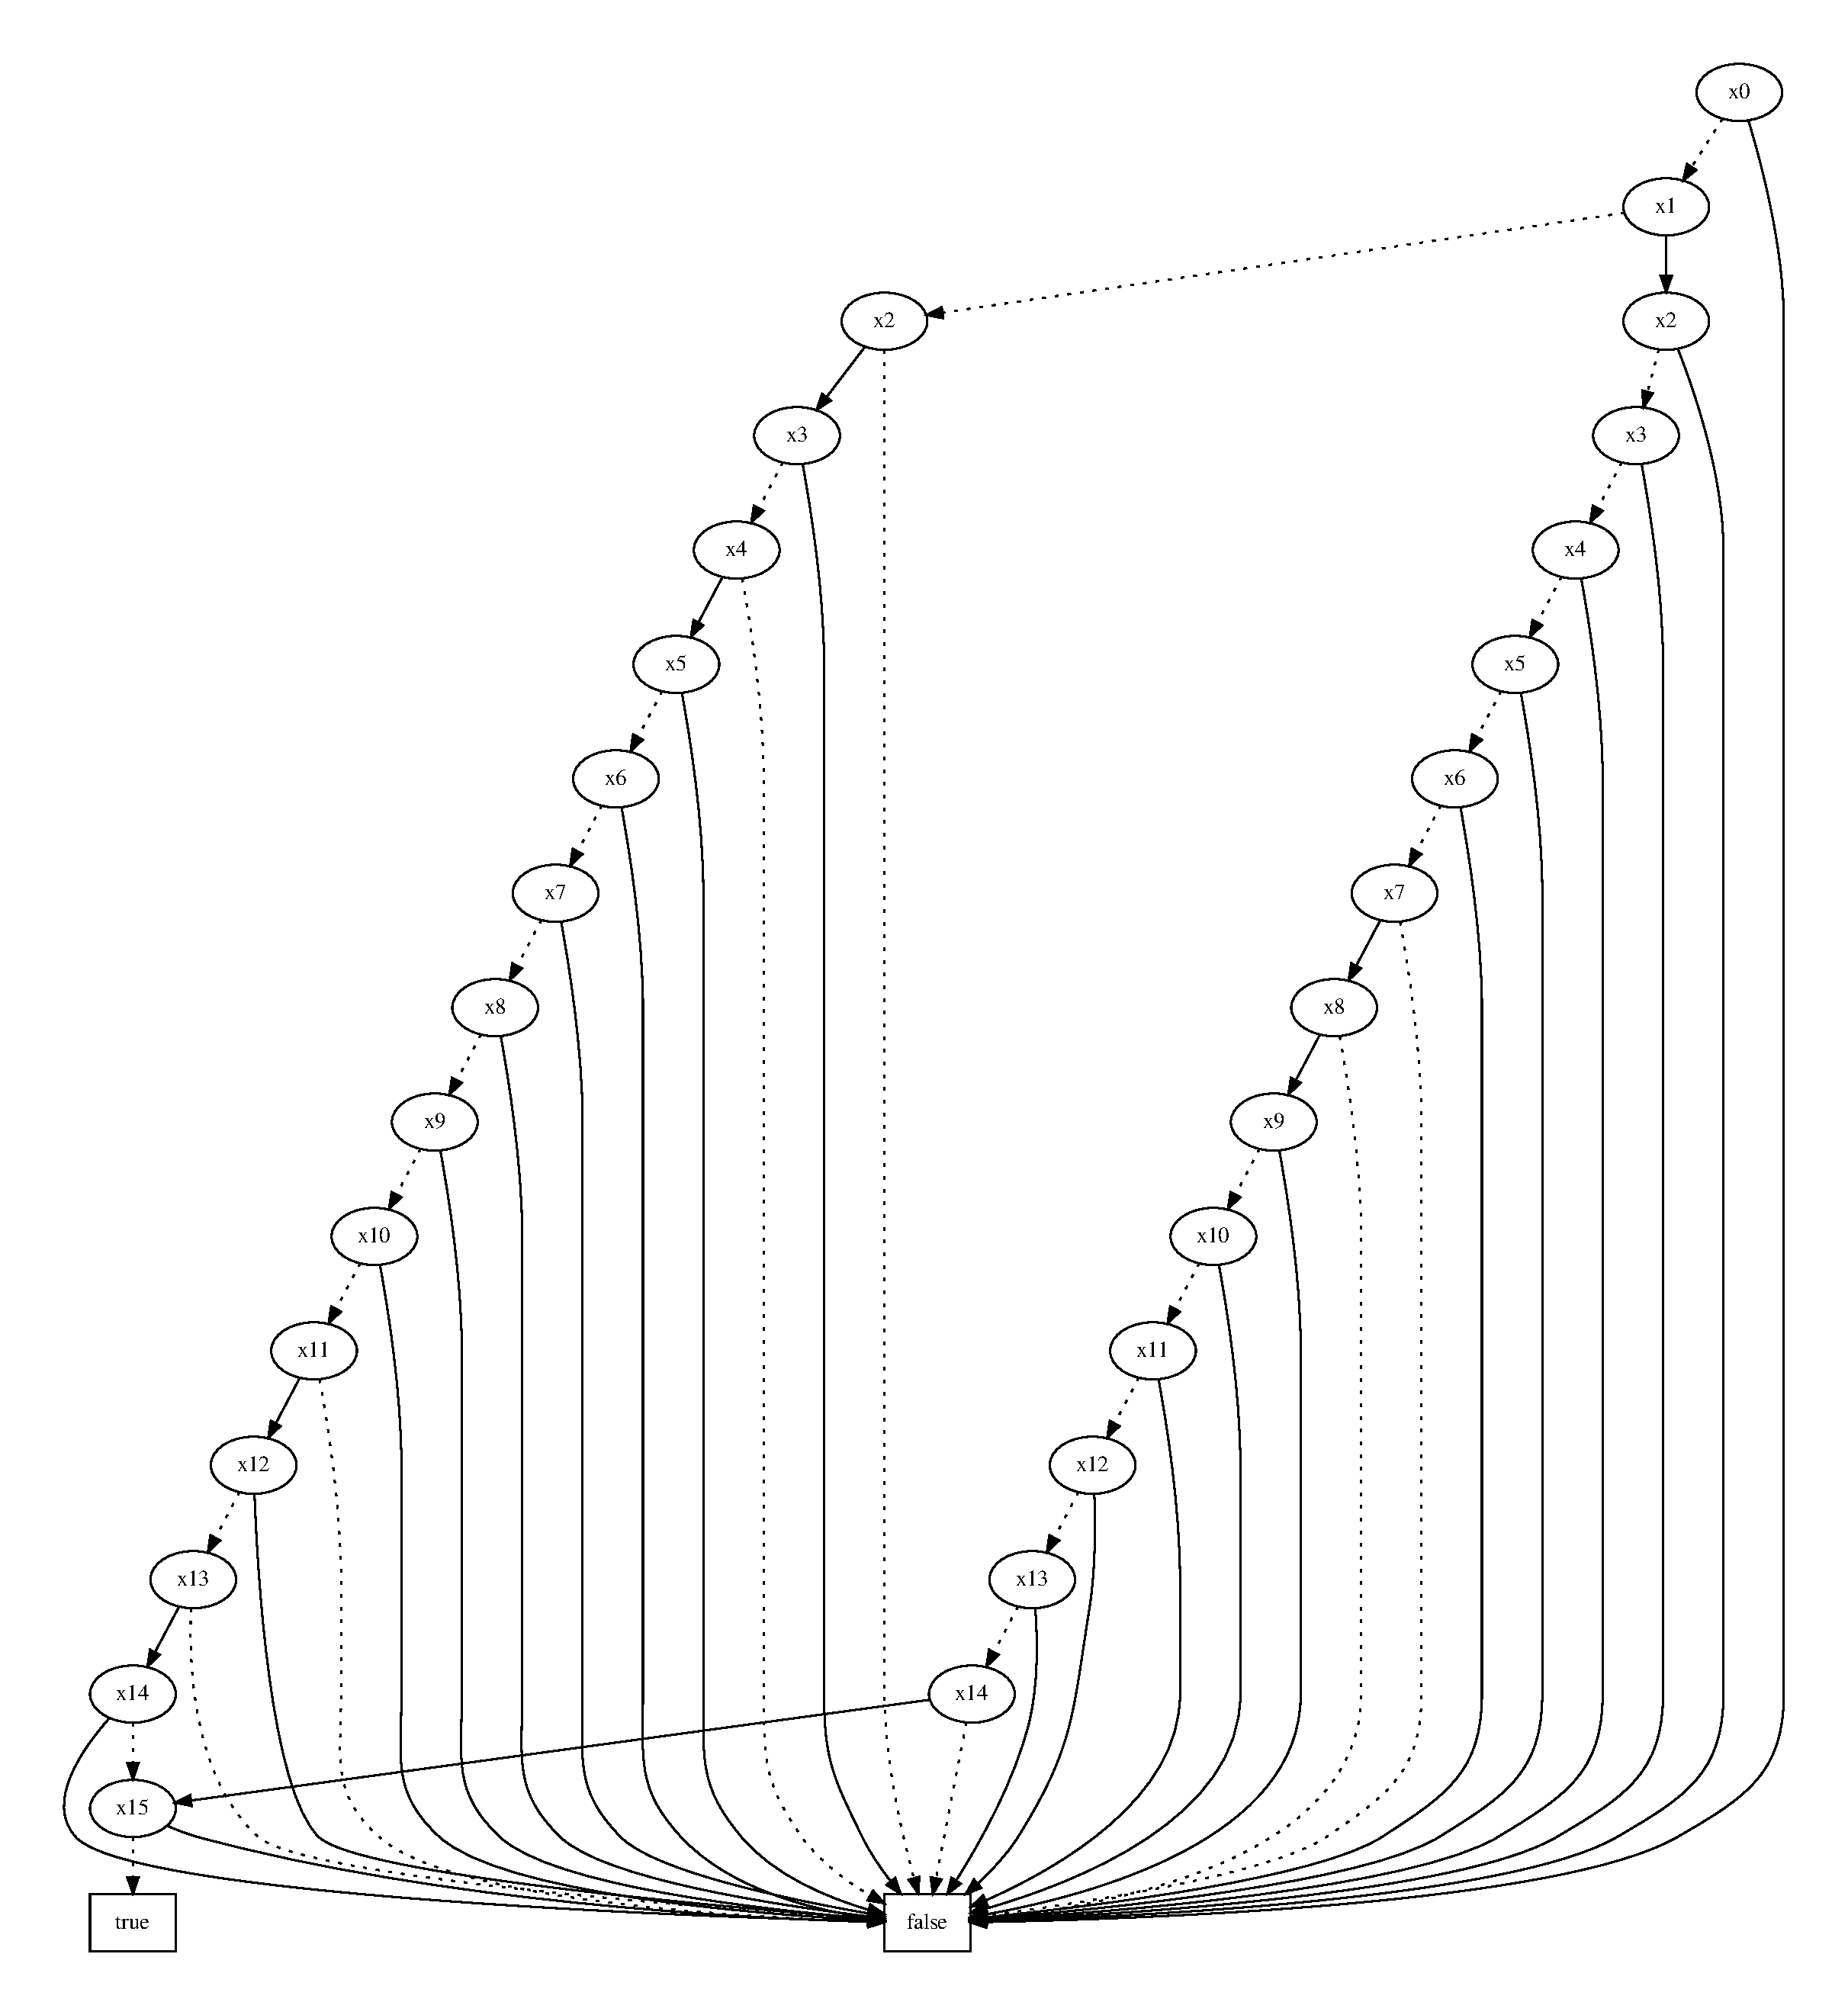
\includegraphics[scale = 0.18]{exemple/queen_4.pdf}
\end{figure}

Avec un total de 2 solutions.\\

La raison pour laquelle ce Sat-solveur n'est pas utilisé est que, bien que la compléxité de l'algorithme ANYSAT soit linéaire, la fonction BUILD est de compléxité exponentielle.

\section{Correction et Equivalence de la combinatoire de circuit}

Lorsque l'on a le ROBDD d'une formule, il est assez facile de voir qu'elles sont les distributions de valeur de vérité qui la satisfaite.\\
Donc une des principales utilisations des ROBDD et pour la correction ou équivalence de circuit (logique).\\

En effet, il est assez évident de voir qu'un circuit logique peut être représenté par une formule.\\
Les entrées sont les variables et les portes les opérations logiques (souvent unaire comme la porte 'NON', ou binaire comme les portes 'OR', 'AND', 'NOR', 'XOR' ...).\\

Comme par exemple : un Circuit d'équivalence \\

\begin{figure}[h]
  \begin{circuitikz}[shorten >=1pt,node distance=0.5cm]
    \node[and port](AND) at (3,2) {\hspace{-1em}and};
    \node[nor port](NOR) at (3,0) {\hspace{-0.8em}nor};
    \node[or port] (OR) at (5,1) {\hspace{-0.6em}or};
    \node		    (X) at (0,2) {$x$};
    \node            (Y) at (0,0) {$y$};
    \node            (Z) at (6,1) {$z$};
    \node[fill,circle,inner sep=0pt,minimum size=1pt]            (XP) at (1.1,2) {\textbullet};
    \node[fill,circle,inner sep=0pt,minimum size=1pt]            (YP) at (0.7,0) {\textbullet};

    \draw (X) -* (XP);
    \draw (XP) |- (AND.in 1);
    \draw (XP) |- (NOR.in 1);
    \draw (Y) -* (YP);
    \draw (YP) |- (AND.in 2);
    \draw (YP) |- (NOR.in 2);
    \draw (AND.out) |- (OR.in 1);
    \draw (NOR.out) |- (OR.in 2);
    \draw (OR.out) |- (Z);
	
  \end{circuitikz}
\end{figure}

De formule : $((x \wedge y) \vee (\neg(x \vee y)))$

\begin{figure}[h]
      \begin{tikzpicture}[shorten >=1pt,node distance=1cm]
\node 			(N) at (0,3)		{ROBDD d'ordre : $x < y$};
  \node[state]		   (X) at (0,2)         {$x$};
  \node[state]         (Y0) at (-1,1)		 {$y$};
  \node[state]         (Y1) at (1,1)		 {$y$};
  \node[state]         (Z0) at (-1,-0.5)		 {$0$};
  \node[state]         (Z1) at (1,-0.5)		 {$1$};


  \path[->,>=stealth', dashed] 
        (X) edge              node {} (Y0)
        (Y0) edge              node {} (Z1)
        (Y1) edge              node {} (Z0);
		
  \path[->,>=stealth'] 
        (X) edge              node {} (Y1)
		(Y0) edge              node {} (Z0)
		(Y1) edge              node {} (Z1);
	
\end{tikzpicture}
\end{figure}

Pour la traduction des circuits en ROBDD sans passer par la formule revient à créer des ROBDDs pour chaque variables :

\begin{figure}[h]
      \begin{tikzpicture}[shorten >=1pt,node distance=1cm]
\node 			(N) at (0,2.5)		{Variable : x};
  \node[state]		   (X) at (0,1.5)         {$x$};
  \node[state]         (Y) at (-1,0)		 {$0$};
  \node[state]         (Z) at (1,0)		 {$1$};


  \path[->,>=stealth', dashed] 
		(X) edge              node {} (Y);
		
  \path[->,>=stealth'] 
        (X) edge              node {} (Z);
	
\end{tikzpicture}
\end{figure}

Puis d'appliquer la fonction APPLY en fonction des portes logiques utiles.\\

\newpage

\begin{lstlisting}
let apply (op : node->node->node) (u1 : node) (u2 : node) : node =
    let g = Hashtbl.create (map_size*map_size) in
    let rec aux (u1 : node) (u2 : node) : node =
      if Hashtbl.mem g (u1, u2) then Hashtbl.find g (u1, u2)
      else
        let u =
          if unite u1 && unite u2 then op u1 u2
          else if var u1 = var u2 then              (* c1 *) 
            mk (var u1)
              (aux (low u1) (low u2)) 
              (aux (high u1) (high u2))
          else if var u1 < var u2 then              (* c2 *) 
            mk (var u1)
              (aux (low u1) u2) 
              (aux (high u1) u2)
          else                                      (* c3 *)
            mk (var u2)
              (aux u1 (low u2)) 
              (aux u1 (high u2))
        in 
        Hashtbl.add g (u1, u2) u;
        u
    in
    aux u1 u2
\end{lstlisting}

APPLY est un fonction qui nous permet de réunir deux ROBDD par un opérateur $op$ (dans notre cas les différentes portes). Son principe est récursif : On crée un nouveau noeud de $var$ prioritaire par rapport à l'ordre des $var$ des deux noeuds à réunir. On réunit les noeuds $low$ des deux noeuds en fonction de leur priorité dans l'ordre et fait de même pour les $high$. Ces deux nouveaux noeuds sont le $low$ et le $high$ du nouveau noeud. Si les noeuds à réunir sont des $1$ et $0$, on applique l'opérateur.\\

APPLY ne viole pas les règles des ROBDD car elle utilise MK qui gère l'unicité des noeuds et la non-redondance et l'ordre est gèré directement dans l'algorithme avec les conditions $c1, c2, c3$.\\

Utiliser APPLY nous permet alors de juste parcourir le circuit et construire le ROBDD en même temps.\\


Ainsi, vérifier qu'un circuit logique donne les bons résultats devient très simple avec son ROBDD et montrer que deux circuits sont équivalents revient à remarquer que les deux ROBDD sont exactement les mêmes (par unicité des ROBDD).


\newpage

\section{Théorie sur les ordres}

Lors de nos recherches, nous avons remarqué que pour des ordres différents, une même expression Booléenne pouvait avoir des ROBDDs différents.\\
Nous avons observé que pour certaine expression le nombre de noeud des ROBDD pouvait considérablement diminuer en fonction de l'ordre choisi a tel point que l'execution de BUILD n'était plus qu'en $O(n)$ au lieu de $2^n$ (où $n$ est le nombre de variable de l'expression).\\

\begin{figure}[h]
      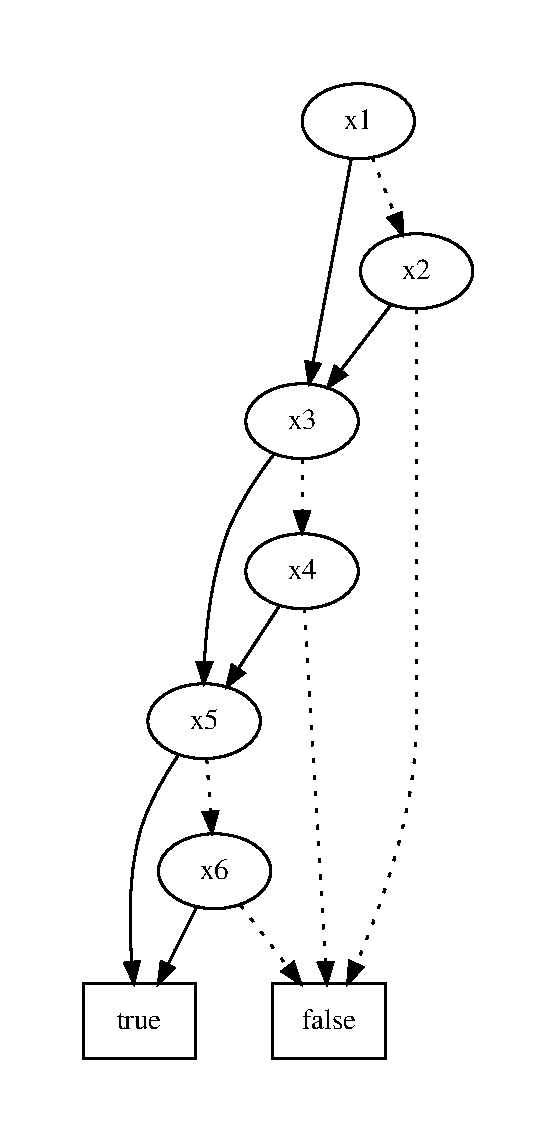
\includegraphics[scale = 0.5]{exemple/bon_Ordre.pdf}
      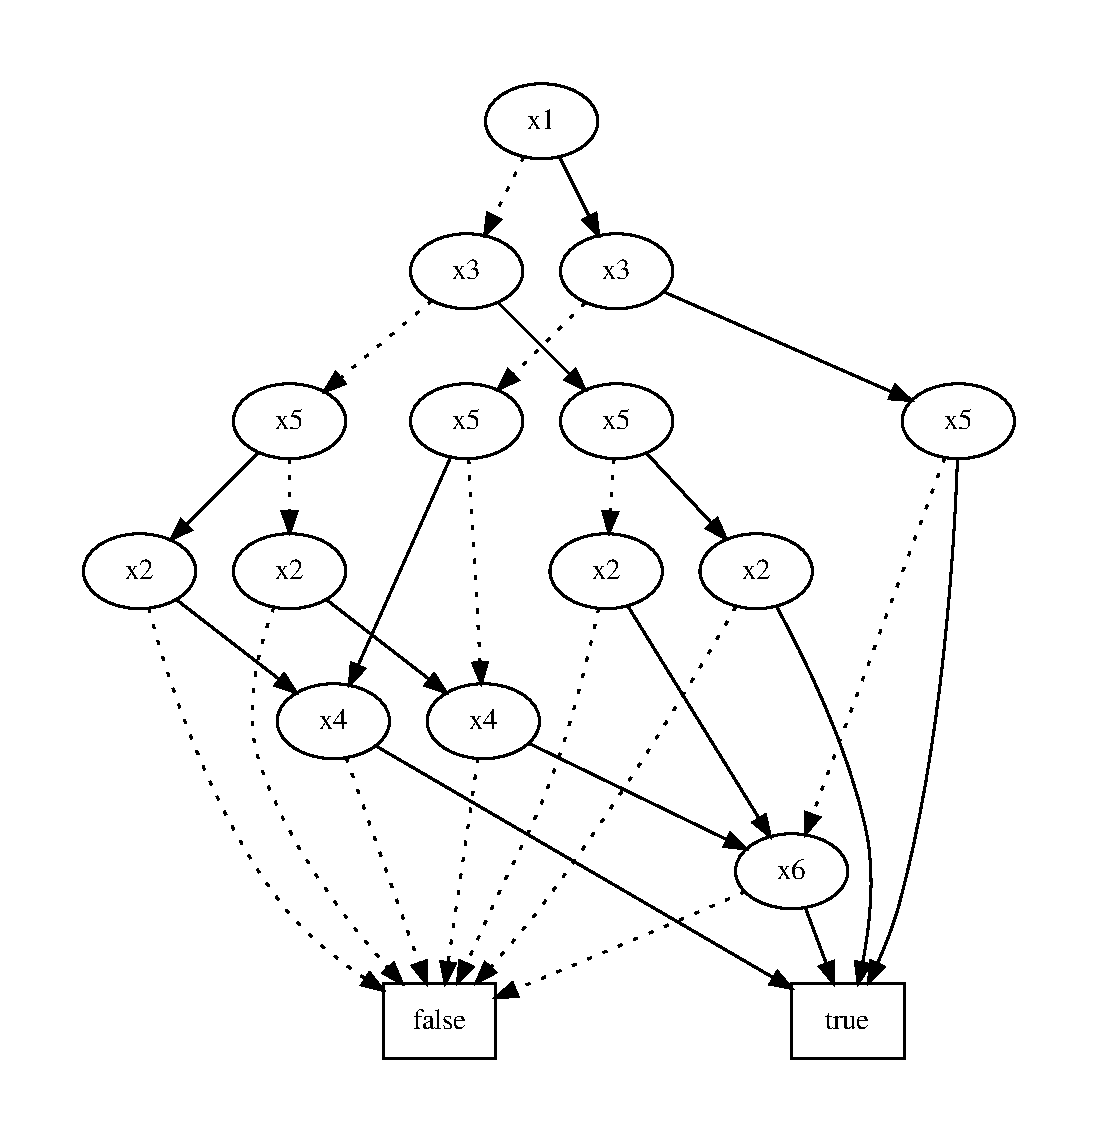
\includegraphics[scale = 0.5]{exemple/mauvais_Ordre.pdf}
    \caption{ROBDD d'ordre $x_1<x_2<x_3<x_4<x_5<x_6$ puis d'ordre $x_1<x_3<x_5<x_2<x_4<x_6$ de la formule : $ (x_1 \vee x_2) \wedge (x_3 \vee x_4) \wedge (x_5 \vee x_6)$}
\end{figure}

Nous nous sommes donc demandé si pour chaque expression Booléenne il existe un ordre qui permet d'obtenir, via la fonction BUILD, un ROBDD en temps linéaire, et dans le cas où il existe, comment le trouver.\\

% L'ordre existe-t-il ?

Malheuresement, il s'avère que trouver le meilleur ordre (celui qui donne un nombre minimal de noeud dans le ROBDD) est un problème NP-Complet % NP-Dur
ce qui ne permet pas de réduire la compléxité de la fonction BUILD.


%%%%% Conclusion %%%%%%%
\chapter*{Conclusion}
\addcontentsline{toc}{chapter}{Conclusion}
L'utilisation des \adbocs est une nouvelle approche des \expp qui est très intéressante. Ce projet a été une première approche à la recherche en mathématique et en informatique sur les \expps.\\
De plus, on a pu voir la complexité de trouver une méthode de résolution \textit{SAT} même si cet algorithme n'est pas adapté pour être un \textit{SAT-solveur}.\\
On a du faire un travail de recherche sur les différents ordres possibles pour une \expp pour voir s'il n'existait pas un ordre qui permettrait de construire un arbre en temps polynomiale.\\
Si un tel ordre existait, on pourrait construire l'arbre en temps polynomiale et ensuite trouver une solution en temps linéaire : ce qui pourrait être très intéressant pour un Sat-solveur.\\
On a vu que pour une même \expp, on peut avoir deux ordres différents nous donnant un nombre de nœud totalement différent.\\
Ceci est une toute nouvelle approche possible qu'on a pu avoir.\\
Cependant, l'utilisation d'un \adboc est surtout pour déterminer si deux \expps sont équivalentes : comme on construit un arbre canonique, on obtient, pour un même ordre, le même arbre si les deux\expps sont équivalentes.\\
Ensuite, un \adboc permet aussi de représenter une \expp sous une forme plus compréhensible par un humain.\\
Nous tenions à remercier Monsieur Sedki Boughattas qui nous a encadré pour ce projet. Nous avons été très intéressé par ce sujet.
%%%%% Bibliographie %%%%%%%
\chapter*{Bibliographie}
\addcontentsline{toc}{chapter}{Bibliographie}
Article de Henrik Reif Andersen : \textit{An Introduction to Binary Decision Diagrams}

\end{document}
